\chapter{Application}
\label{chapter:application}
In this chapter we are going to have an in-depth look at the architecture of our application - \textbf{ExtWatcher}, that represents a solution for the enunciated problem in this thesis.


\section{Design}
\label{section:design}
\textit{ExtWatcher} is a software application assembled from multiple components using different technologies (see Figure \ref{deployment}). In the following we will introduce you into it's implementation design starting from the low level and we will explain what role each component plays in the context of providing a truly effective security solution. 

\begin{figure}[H]
	\centerline{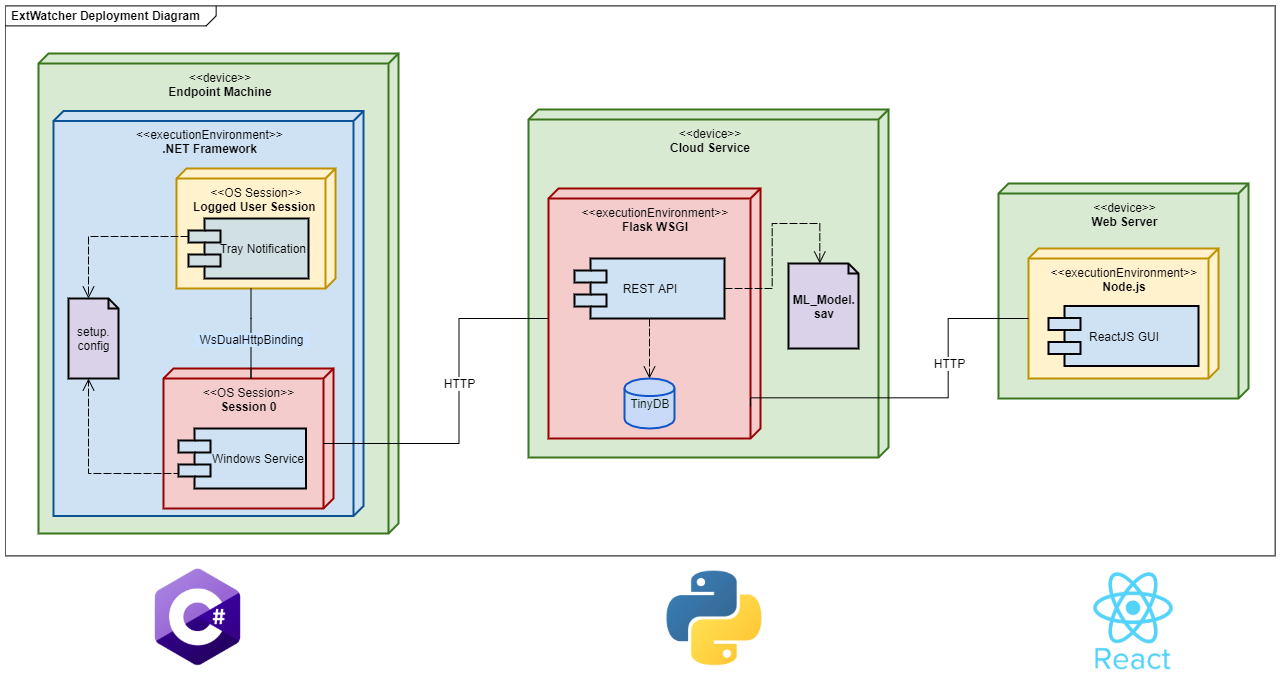
\includegraphics[scale=0.4]{figures/deployTech.png}}  
	\caption{Deployment Diagram of the application and used technologies}
	\label{deployment}
\end{figure}

The core of the entire software application is the \textit{Cloud Analyzer}, which provides the security measure against malicious PDF documents. ExtWatcher has two different, independent approaches for getting access to the Cloud Analyzer. 

\begin{itemize}
	\item The first one implies automatic file detection and requires the installation of \textit{ExtWatcher Service}, which will establish a connection through HTTP to the Cloud Analyzer and will instantly remove detected malicious files from the user's computer.
	\item The second approach is an \textit{out-of-the-box} functionality, the user being able to analyze a file by accessing the Cloud Analyzer Dashboard (web graphical user interface) and entering the URL of the file. The dashboard submits the URL to the Cloud Analyzer and the later downloads the file, classifies it and sends back the verdict. This solution is fit for mobile devices, as it requires no additional installation, ExtWatcher Service being currently supported just on Windows OS.
\end{itemize}

In order to properly work, our application requires permanent Internet connection, because the core of analysis is remotely located. The advantage of this is the fact that Cloud servers are better at applying Machine Learning models for malware detection, thereby reducing the workload on personal computers. 


\section{ExtWatcher Service}
\label{section:winService}
This section will describe how the Windows Service manages to simplify the user responsibility and to automate the task of detection and uploading of PDF files to our analysis engine. As previously mentioned, this is not a mandatory component, rather just a help utility for users whose computers work on Windows platform. However this tool itself integrates two separate executables (the service and the app aimed to send system notifications), each with its own configuration files. Of course, field knowledge is required in order to correctly configure this tool and to let it run errorlessly. To solve this problem and to make \textit{ExtWatcher Service} accessible for everyone, we created a Setup Installation File, which packages all the necessary files and installation information into a \textit{MSI} file. The user should just launch the installer executable to get \textit{ExtWatcher Service} properly working on their computers. Under the hood, the used Windows Installer, unpackages those two applications and their configuration files, moves them to the corresponding installation folder, writes the suitable registry keys to set the \textit{Tray Notification App} to launch at the user's login, installs the service into Windows Service Manager and starts the utility right after the installation is done. \par
After ExtWatcher Service is up, it should guarantee the security of the user's computer. By default, the filesystem's \texttt{C:\textbackslash} and \texttt{D:\textbackslash} disks are monitored. However, modifying the \texttt{setup.config} configuration file found in the installation folder of the software, allows to add new filepaths for continuous monitoring. In this way the user can be sure, that once he downloads any PDF file to his computer, the integrity of the system is protected by our application. Basically the Windows Service detects that a new file of type PDF was downloaded, blocks and hides it, so that the user can not access the file until it is not scanned. Next, the Windows Service submits the file to the remote server for analysis. While waiting for the response, it sends an event to the \textit{Tray Notification Application}, which is responsible for pushing System Notifications to the user, saying that the downloaded PDF is being scanned (see Figure \ref{screenshot:notification}). After the analysis response in JSON format is caught by Windows Service, it takes the corresponding action on the PDF file, based on the \textit{verdict} extracted from JSON. 

\begin{itemize}
	\item \texttt{benign} - this verdict means that the Windows Service can take out the applied restrictions (block and hide) from the file.
	\item \texttt{malicious} - Windows Service should immediately remove the file from the disk.
\end{itemize}

The above described flow can be visualized in Fig. \ref{sequence}. The implementation design of ExtWatcher Service takes in consideration further evolution of our product. So, it can be easily configured using same \texttt{setup.config} to monitor more file extensions, when the Cloud Analyzer will contain support for analyzing more file formats.

\begin{figure}[H]
	\centerline{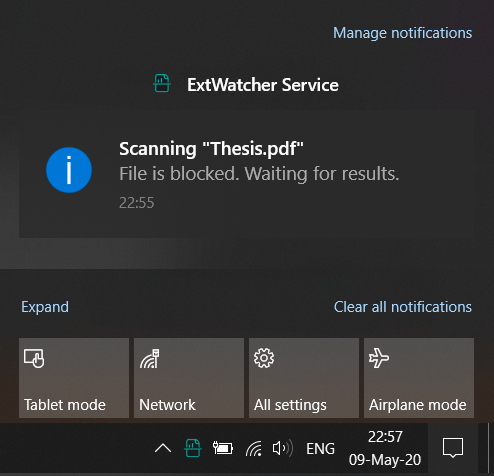
\includegraphics[scale=0.55]{figures/notification.png}}  
	\caption{Screenshot of the System Notification sent by ExtWatcher Service}
	\label{screenshot:notification}
\end{figure}

\newpage

\begin{figure}[H]
	\centerline{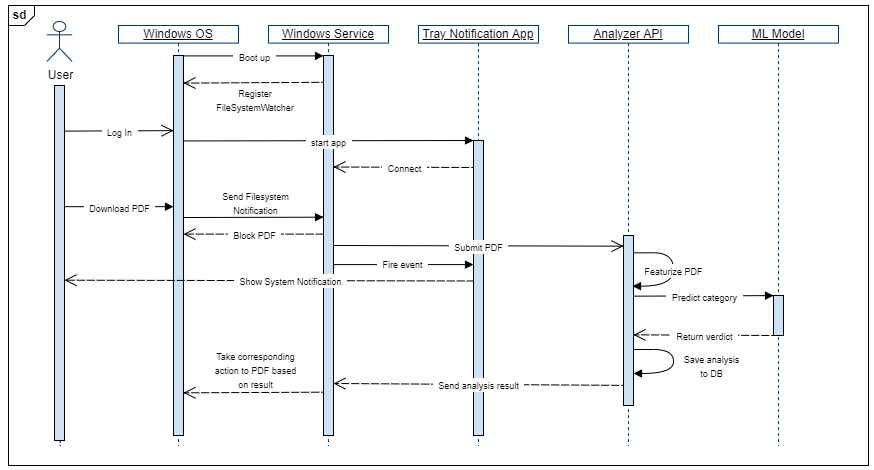
\includegraphics[scale=0.55]{figures/sequence.png}}  
	\caption{Sequence Diagram showing interaction between User, Windows Service and Cloud Analyzer}
	\label{sequence}
\end{figure}


\section{Cloud Analyzer}
\label{section:cloudApi}
Next we will finally cover the core of our product - the Cloud Analyzer. As mentioned in section \ref{section:design}, there are multiple ways to access the core, as it is a Cloud based solution. The first two methods are straightforward and make the use of the Cloud application intuitive. Nevertheless we designed our API keeping in mind the REST\footnote{REpresentational State Transfer (REST)} architecture. As effect, we have a strong separation between the server and client side, thus giving the oportunity to our API to be integrated in multiple ways. Beside the \textit{visual} method (web Dashboard Interface) and the \textit{automation} method (ExtWatcher Service), this framework can be adapted to more use-cases. The custom client can access it via the exposed REST interface, no limitations being currently applied. This independence of the Cloud Analyzer assured by the RESTful design makes it flexible and portable, permitting to configure it in different types of environments. It was not the purpose of this thesis to deploy the framework to any Cloud service, but it was a main goal to achieve it's portability and ease of configuration. \par 
As it was clear that our framework is going to be a resource for just retrieving data from it, without requiring any information about client's state, we fulfilled another REST paradigm - \textit{Stateless}. Due to this, the application achieves scalability and performance, the communication between client and server being simple and not relying on implementation of interfaces. The pattern of interchanging data is based on requests and responses, where the HTTP communication protocol is used. \par
In order to retrieve information about a PDF file, the \textit{ExtWatcher Service} uses a \code{POST} HTTP method to upload the file to the framework. The request contains two main parts: \textit{Header}, which contains all the information about the request, in our case the content type of the body: \texttt{application/pdf}; and the \textit{Body}, which basically contains the content of the uploaded file. Specifying the content type is really importantat, because that ensures that the server is able to process the request. Once the PDF is uploaded to the server, first of all, the MD5 hash of the file is calculated to check in the database if the same file was not already analyzed. If the hash is not found, the file is being analyzed by applying the ML model for predicting the file maliciousness. The result together with a HTTP status code (\textit{200} - for successful process; \textit{400} - for bad request) is then sent back as response. \par
The web Dashboard's integration with the Cloud Analyzer is a bit different. Mostly it accesses the server in order to retrieve stored information about previous analyses. That is achieved via \code{GET} HTTP methods. The response is in JSON format and can be easily processd by the Javascript client in order to offer an intuitive visualization of it. An in-depth particularization of all exposed methods from our framework can be studied in the Table \ref{table:rest}.

\begin{table}[H]
	\caption{REST Resources of the Cloud Analyzer API}
	\label{table:rest}
	\centering
	\begin{tabular}{p{5cm} | c | p{9cm}}
		\toprule
		
		\textbf{Resource} & \textbf{Method} & \textbf{Purpose} \\
		\hline 
		\texttt{/api/file-upload} & \code{POST} & Uploading files for analysis  \\
		\hline
		\texttt{/api/url-submit} & \code{POST} & Submitting URL to a file that should be downloaded and analyzed  \\
		\hline
		\texttt{/api/feed} & \code{GET} & Retrieve the history of events (who and what kind of analysis type started)  \\
		\hline
		\texttt{/api/analyzed-files} & \code{GET} & Obtain a list of informations about all analyzed files \\
		\hline
		\texttt{/api/search-files} & \code{GET} & Search files using queries for filtering by different file attributes \\
		\hline
		\texttt{/api/extwatcher-service} & \code{GET} & Download ExtWatcher Service Installer\\
		
		\bottomrule
	\end{tabular}
\end{table}

\newpage

		
\section{Dashboard Interface}
\label{section:dashboard}
\textit{ExtWatcher} also offers an intelligent solution for interacting with the Cloud Analyzer API and to visualize the data that passed through it. This is a responsive web Dashboard with the help of which users can interact with the API from any device, be it laptop or smartphone. An overview of the Dashboard capabilities is presented in Figure \ref{usecase}. 

\begin{figure}[H]
	\centerline{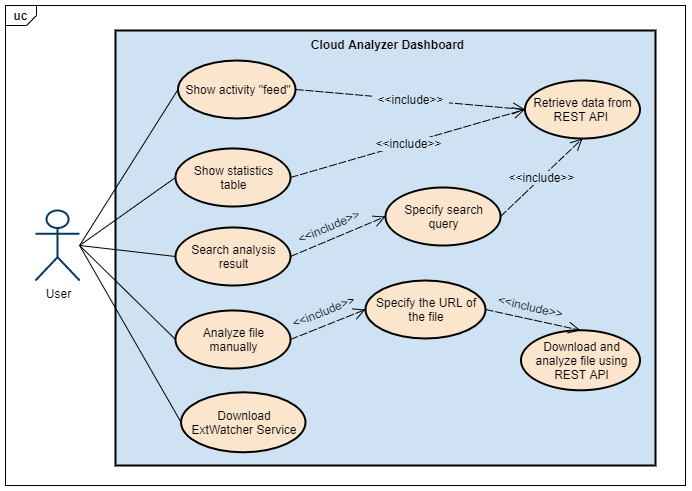
\includegraphics[scale=0.7]{figures/usecaseGUI.png}}  
	\caption{Use Case Diagram showing interaction between User and Cloud Analyzer using web GUI}
	\label{usecase}
\end{figure}

It was implemented separately from the server, so it calls just the API methods it requires, without being forced to implement a concrete server interface. The connection between these two is established via HTTP protocol and mostly the Dashboard works with the \code{GET} methods to access the server's resources (see Table \ref{table:rest}) and to present them to users. At the moment, any user that accesses the Dashboard has the possibility to view statistics about all files ever scanned, including file details such as: filetype, MD5 hash of the file, filename, date when it was scanned and result of analysis (see Figure \ref{screenshot:infotable}). 

\begin{figure}[H]
	\centerline{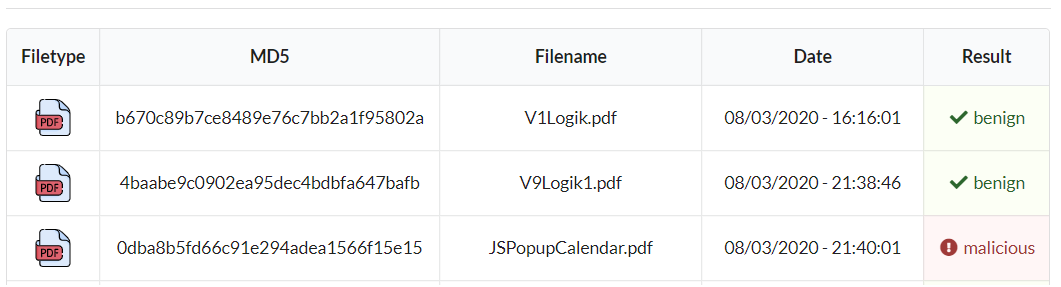
\includegraphics[scale=0.6]{figures/infotable.png}}  
	\caption{Screenshot of the ExtWatcher Dashboard table of file informations}
	\label{screenshot:infotable}
\end{figure}

Also the dashboard presents a "feed", that serves as a history of using the Cloud Analyzer (see Figure \ref{screenshot:feed}). It includes information about how each file came to be analyzed: by being uploaded by the ExtWatcher Service or by manually submitting the URL of the file, as well as information about the IP the file was originated from.

\begin{figure}[H]
	\centerline{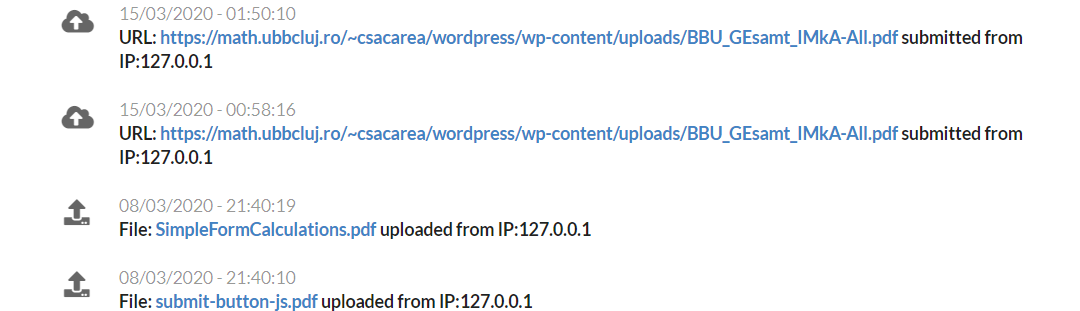
\includegraphics[scale=0.6]{figures/feed.png}}  
	\caption{Screenshot of the ExtWatcher Dashboard activity feed}
	\label{screenshot:feed}
\end{figure}

Of course, to simplify the interaction with this web application, it provides also a \textit{searchbar}. The user can quickly find information about any file, by specifying a basic search query (see Figure \ref{screenshot:searchbar}).

\begin{figure}[H]
	\centerline{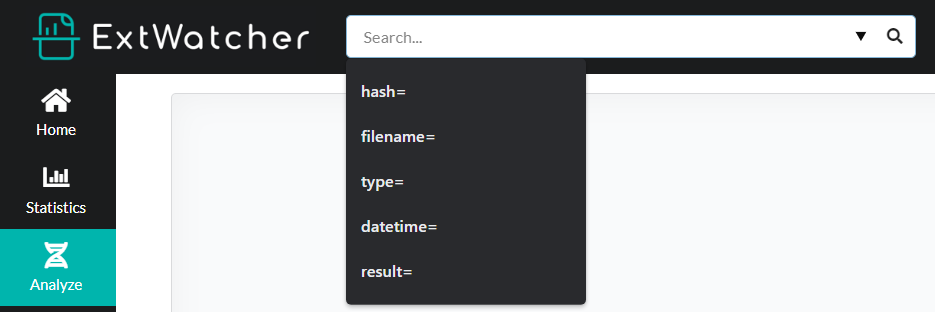
\includegraphics[scale=0.6]{figures/searchbar.png}}  
	\caption{Screenshot of the ExtWatcher Dashboard searchbar and types of search queries}
	\label{screenshot:searchbar}
\end{figure}

For those users who adopt the automatic detection and submission to the Cloud Analyzer approach, using the \textit{ExtWatcher Service}, the Windows Installer can be downloaded directly from the Dashboard (see Figure \ref{screenshot:installer}). 

\begin{figure}[H]
	\centerline{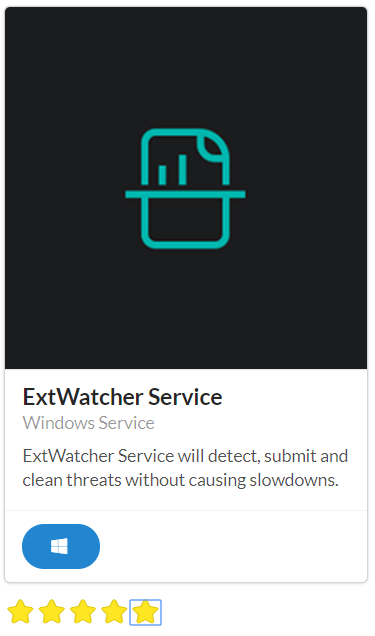
\includegraphics[scale=0.45]{figures/installer.png}}  
	\caption{Screenshot of the ExtWatcher Dashboard download page for ExtWatcher Service Installer}
	\label{screenshot:installer}
\end{figure}

However, we took in consideration the alternative case, when not all users would prefer this method or some just don't have a computer with Windows OS (single OS for which ExtWatcher Service has support yet). There is another method to analyze PDF files directly from the web Dashboard. The user should just specify the URL of the file he wants to analyze and the rest of the workload is taken by the Cloud Analyzer. In this way, the user can be confident that no PDF file can harm his device, because it is first downloaded by the Cloud Analyzer and is analyzed on a remote, safe environment. After the analysis result is showed, the user can decide what to do with that file (see Figure \ref{screenshot:analyze}).

\begin{figure}[H]
	\centerline{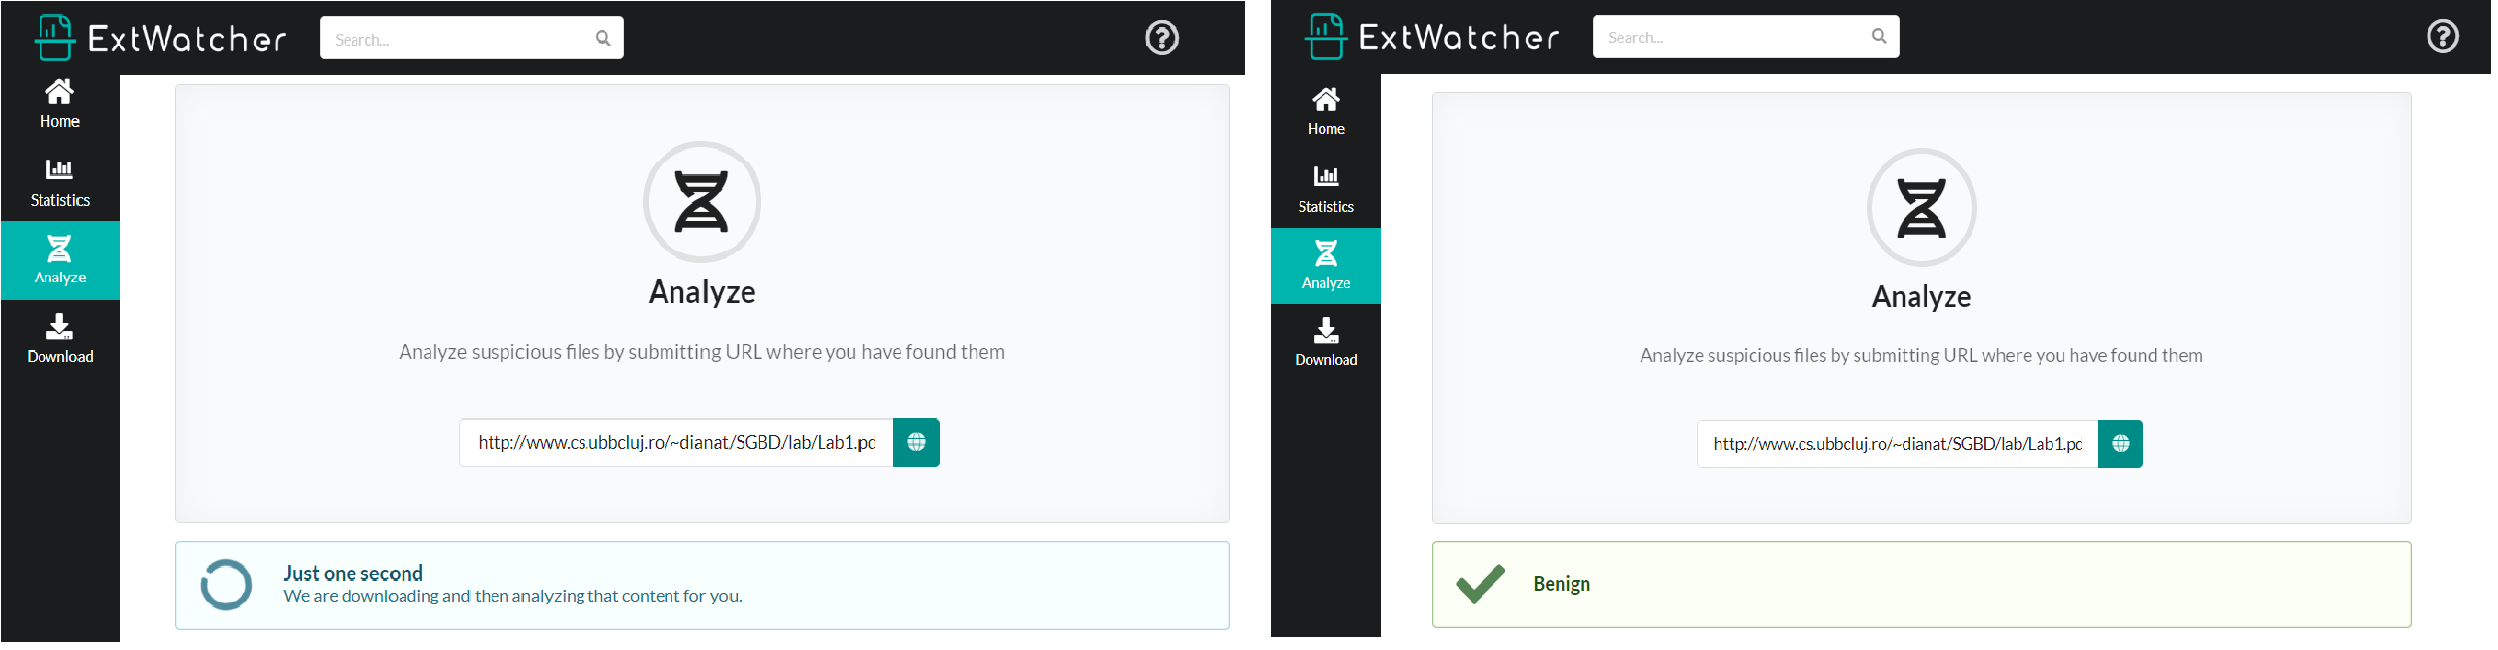
\includegraphics[scale=0.35]{figures/analyze.png}}  
	\caption{Screenshot of the ExtWatcher Dashboard analyze page}
	\label{screenshot:analyze}
\end{figure}